\documentclass{article}

\usepackage[T1]{fontenc}
\usepackage[utf8]{inputenc}
\usepackage{times}

\usepackage[font=small,labelfont=bf,tableposition=top]{caption}
\usepackage{graphicx}
\usepackage{natbib} 

\usepackage{amsmath}
\usepackage{amsfonts}
\usepackage{amssymb}
\usepackage{color, soul}
\usepackage{hyperref}
\usepackage{algorithmicx}
\usepackage{algpseudocode}
\usepackage{subfigure}
\usepackage{stmaryrd}

\renewcommand{\vec}[1]{\boldsymbol{{#1}}} 
\newcommand{\duesoon}[1]{{\sethlcolor{green}\hl{#1}}}
\usepackage{mathrsfs}


\newtheorem{theorem}{Theorem}
\newtheorem{acknowledgement}[theorem]{Acknowledgement}
\newtheorem{algorithm}[theorem]{Algorithm}
\newtheorem{axiom}[theorem]{Axiom}
\newtheorem{case}[theorem]{Case}
\newtheorem{claim}[theorem]{Claim}
\newtheorem{conclusion}[theorem]{Conclusion}
\newtheorem{condition}[theorem]{Condition}
\newtheorem{conjecture}[theorem]{Conjecture}
\newtheorem{corollary}[theorem]{Corollary}
\newtheorem{criterion}[theorem]{Criterion}
\newtheorem{definition}[theorem]{Definition}
\newtheorem{example}[theorem]{Example}
\newtheorem{exercise}[theorem]{Exercise}
\newtheorem{lemma}[theorem]{Lemma}
\newtheorem{notation}[theorem]{Notation}
\newtheorem{problem}[theorem]{Problem}
\newtheorem{proposition}[theorem]{Proposition}
\newtheorem{remark}[theorem]{Remark}
\newtheorem{solution}[theorem]{Solution}
\newtheorem{summary}[theorem]{Summary}
\newenvironment{proof}[1][Proof]{\textbf{#1.} }{\ \rule{0.5em}{0.5em}}

\newtheorem{guess}{Definition}
\newcommand{\comment}[1] {}
\newcommand{\Norder} {N}
\newcommand{\order}{\mathcal{O}}
\newcommand{\Npoints} {N_p}
\newcommand{\Nfaces} {N_{f}}
\newcommand{\Nelements} {N_e}

\newcommand{\eps}{\varepsilon}
\newcommand{\Dweak}{\wt{D}}
\newcommand{\diff}[2] {\frac{\partial #1}{\partial #2}}
\newcommand{\dxx}[2] {\frac{\partial^2 #1}{\partial {#2}^2}}
\newcommand{\difft}[2] {\frac{d #1}{d #2}}
\newcommand{\dxxt}[2] {\frac{d^2 #1}{d {#2}^2}}
\newcommand{\lagrange}[1] {\frac{d #1}{dt}}
\newcommand{\lebesgue}{\parallel I \parallel}
\newcommand{\polysp}{\mathcal{P}_N}
\newcommand{\laplacian}{\nabla^2}
\newcommand{\divergence}{\nabla \cdot}
\newcommand{\inte}{\int_{\mbox{\footnotesize ${\Omega_e}$}}}
\newcommand{\intb}{\int_{\mbox{\footnotesize ${\Gamma_e}$}}}
\newcommand{\intce}{\int_{\mbox{\footnotesize ${\widehat{\Omega}_e}$}}}
\newcommand{\intcb}{\int_{\mbox{\footnotesize ${\widehat{\Gamma}_e}$}}}
\newcommand{\intg}{\int_{\mbox{\footnotesize ${\Omega}$}}}
\newcommand{\intgb}{\int_{\mbox{\footnotesize ${\Gamma}$}}}
\newcommand{\intv}{\int_{\mbox{\footnotesize ${\sigma}$}}}
\newcommand{\sumv}{\sum_{K=1}^{N_{\mathrm{lev}}}}
\newcommand{\sumk}{\sum_{L=1}^{K}}
\newcommand{\sumN}{\sum_{i=1}^{N+1}}
\newcommand{\half}{\frac{1}{2}}
\newcommand{\inti}{\int_{\mbox{\footnotesize\sf I}}}
\newcommand{\intbd}{\oint_{\mbox{\footnotesize ${\delta}$\sf D}}}
\newcommand{\intbi}{\oint_{\mbox{\footnotesize ${\delta}$\sf I}}}
\newcommand{\ldnorm}[1]{\left\| #1 \right\|_{\mbox{\footnotesize \sf D}} }
\newcommand{\lonorm}[1]{\left\| #1 \right\|_{\Omega}}
\newcommand{\spc}[1]{\mbox{\sf #1}}
\newcommand{\ope}[1]{{\cal #1}}
\newcommand{\mt}[1]{{\rm #1}}
\newcommand{\dis}{\displaystyle}
\newcommand{\ve}{\varepsilon}
\newcommand{\ov}{\overline}
\newcommand{\wt}{\widetilde}
\newcommand{\wh}{\widehat}
\newcommand{\Dhat}{\widehat{D}}
\newcommand{\be}{\begin{equation}}
\newcommand{\ee}{\end{equation}}
\newcommand{\bea}{\begin{eqnarray*}}
\newcommand{\eea}{\end{eqnarray*}}
\newcommand{\Jace}{J^{(e)}}
\newcommand{\Jacl}{J^{(l)}}
\def\bepsilon{\mbox{\boldmath $\epsilon $}}
\def\bpsi{\mbox{\boldmath $\psi $}}
\def\bphi{\mbox{\boldmath $\phi $}}
\def\bmu{\mbox{\boldmath $\mu $}}
\def\Et{ \tilde{E} }
\def\Ht{ \tilde{H} }
\def\sdot{ \dot{\sigma} }

\newcommand{\fstar}{f^{(*)}}

\DeclareMathOperator{\Span}{span}
\DeclareMathOperator{\Dim}{dim}

\newcommand{\polyquad}{\mathcal{Q}_{N}}
\newcommand{\polyP}{\mathcal{P}_{N}}
\newcommand{\polyPnpm}{\mathcal{P}_{(N+M)}}
\newcommand{\polyPd}{\mathcal{P}_{d}}
\newcommand{\polyPnm}{\mathcal{P}_{N,M}}
\newcommand{\polyPn}{\mathcal{P}_{N,0}}
\newcommand{\transpose}{^{\mathcal{T}}}

\newcommand{\vecQ}{\vec{Q}}
\newcommand{\vecQe}{\vec{Q}^{(e)}}
\newcommand{\vecFe}{\vec{\mathcal{F}}^{(e)}}
\newcommand{\statevec}{\vec{Y}}
\newcommand{\statevecN}{\vec{Y}_N^{(e)}}
\newcommand{\statestage}{\vec{\mathcal{Y}}}
\newcommand{\Ftensor}{\vec{F}(\qvector)}
\newcommand{\FtensorN}{\vec{F}\left( \qvectorN \right)}
\newcommand{\FtensorStar}{\vec{F}\left( \qvector_N^{(e,k)} \right)}
\newcommand{\Svector}{S(\qvector)}
\newcommand{\SvectorN}{S \left( \qvectorN \right)}
\newcommand{\qref}{\vec{q}_0}
\newcommand{\qvectorb}{\vec{q}_b}
\newcommand{\qtt}{\vec{q}_{tt}}
\newcommand{\qhat}{\widehat{\vec{q}}}
\newcommand{\qhatb}{\widehat{\vec{q}}_b}
\newcommand{\qelem}{q^{(e)}}
\newcommand{\rhoref}{\rho_0}
\newcommand{\piref}{\pi_0}
\newcommand{\Thetaref}{\Theta_0}
\newcommand{\Gref}{G_0}
\newcommand{\Tref}{T_0}
\newcommand{\thetaref}{\theta_0}
\newcommand{\Pref}{{P}_0}
\newcommand{\Eref}{{E}_0}
\newcommand{\Href}{{h}_0}
\newcommand{\rhohat}{\widehat{\rho}}
\newcommand{\pihat}{\widehat{\pi}}
\newcommand{\Phat}{\widehat{P}}
\newcommand{\uvechat}{\widehat{{\mbox{\boldmath$u$\unboldmath}}}}
\newcommand{\uhathat}{\widehat{\widehat{{\mbox{\boldmath$u$\unboldmath}}}}}
\newcommand{\Uhat}{\widehat{{\mbox{\boldmath$U$\unboldmath}}}}
\newcommand{\Uhathat}{\widehat{\widehat{{\mbox{\boldmath$U$\unboldmath}}}}}
\newcommand{\thetahat}{\widehat{\theta}}
\newcommand{\Thetahat}{\widehat{\Theta}}
\newcommand{\Ehat}{\widehat{E}}
\newcommand{\uhat}{\widehat{u}}
\newcommand{\vhat}{\widehat{v}}
\newcommand{\what}{\widehat{w}}
\newcommand{\pitt}{\pi_{tt}}
\newcommand{\rhott}{\rho_{tt}}
\newcommand{\Ett}{E_{tt}}
\newcommand{\Utt}{\vec{U}_{tt}}
\newcommand{\uvectt}{\vec{u}_{tt}}
\newcommand{\utt}{u_{tt}}
\newcommand{\vtt}{v_{tt}}
\newcommand{\wtt}{w_{tt}}
\newcommand{\Ptt}{P_{tt}}
\newcommand{\vecPtt}{\vec{P}_{tt}}
\newcommand{\Thetatt}{\Theta_{tt}}
\newcommand{\thetatt}{\theta_{tt}}
%Projector Matrices
\newcommand{\projmatrix}{\vec{\mathcal{P}}}
\newcommand{\qmatrix}{\vec{\mathcal{Q}}}
\newcommand{\pcmatrix}{\vec{\mathcal{P}}_C}
\newcommand{\Cmatrix}{\left(\vec{\mathcal{C}}^{(e,f)}\right)\transpose}
\newcommand{\Dmatrix}{\vec{D}^{(e)}}
\newcommand{\Dwmatrix}{\wt{\vec{D}}^{(e)}}
\newcommand{\Mmatrix}{M^{(e)}}
\newcommand{\Fmatrix}{\vec{F}^{(e,l)}}
\newcommand{\Gmatrix}{\mathcal{G}}
\newcommand{\Umatrix}{\mathcal{U}^{(e,f)}}
\newcommand{\amatrix}{\vec{\mathcal{A}}}
\newcommand{\rmatrix}{\vec{\mathcal{R}}}
%Vectors
\newcommand{\nvector}{\wh{\vec{n}}_{\Gamma}}
\newcommand{\nhat}{\wh{\vec{n}}}
\newcommand{\ivector}{\wh{\vec{i}}}
\newcommand{\jvector}{\wh{\vec{j}}}
\newcommand{\kvector}{\wh{\vec{k}}}
\newcommand{\rvector}{\wh{\vec{r}}}
\newcommand{\svector}{\wh{\vec{s}}}
\newcommand{\tvector}{\wh{\vec{t}}}
\newcommand{\vvector}{\wh{\vec{v}}}
\newcommand{\Qvector}{\vec{Q}}
%Vectors
\newcommand{\ur}{{u}^{(r)}}
\newcommand{\us}{{u}^{(s)}}
\newcommand{\ut}{{u}^{(t)}}
\newcommand{\urtt}{{u}_{tt}^{(r)}}
\newcommand{\ustt}{{u}_{tt}^{(s)}}
\newcommand{\uttt}{{u}_{tt}^{(t)}}
\newcommand{\urhat}{\widehat{u}^{(r)}}
\newcommand{\ushat}{\widehat{u}^{(s)}}
\newcommand{\uthat}{\widehat{u}^{(t)}}
%Other Operators
\newcommand{\grad}{\vec{\nabla}}
\newcommand{\Grad}{\vec{\nabla}}
\newcommand{\Dskew}{\mathcal{D}}

\def\bepsilon{\mbox{\boldmath $\epsilon $}}
\def\bpsi{\mbox{\boldmath $\psi $}}
\def\bphi{\mbox{\boldmath $\phi $}}
\def\bmu{\mbox{\boldmath $\mu $}}
\def\Et{ \tilde{E} }
\def\Ht{ \tilde{H} }
\def\sdot{ \dot{\sigma} }
%\renewcommand{\thetable}{\Roman{table}}
%\renewcommand{\thefigure}{\arabic{figure}}

%\DeclareMathOperator{\Span}{span}
%\DeclareMathOperator{\Dim}{dim}

%Editing Commands
\newcommand{\here}{ \textcolor{red}{YOU ARE HERE}}

%Time-Integration
\newcommand{\dt}{{\Delta t}}
\newcommand\ST{\rule[-0.75em]{0pt}{2em}}
\newcommand{\Sfunction}{\mathcal{S}}
\newcommand{\Lfunction}{\mathcal{L}}
\newcommand{\Nfunction}{\mathcal{N}}

%DG Operators
\newcommand{\average}[1]{ \left\{ #1 \right\} }
\newcommand{\jump}[1]{ \llbracket #1 \rrbracket }

%HDG Matrices
\newcommand{\CCmatrix}{\mathcal{C}^{(e,k)}}
\newcommand{\Jmatrix}{\mathcal{J}^{(e,k)}}
\newcommand{\DDmatrix}{\wt{D}^{(e)}}
\newcommand{\SSvector}{\mathcal{S}(q)}
\newcommand{\cghdg}{cg\underline{\hspace{0.15cm}}to\underline{\hspace{0.15cm}}hdg}
%\newcommand{\ul}{\underline{\hspace{0.15cm}}}
\newcommand{\RRmatrix}{\mathcal{R}}

%Clima specific variables
\newcommand{\etotal}{e^{\mathrm{tot}}}
\newcommand{\Etotal}{E^{\mathrm{tot}}}
\newcommand{\Fvector}{\vec{\mathcal{F}}}
\newcommand{\Pvector}{\vec{\mathcal{P}}}
\newcommand{\Fadv}{\vec{\mathcal{F}}^{\mathrm{adv}}}
\newcommand{\Fndf}{\vec{\mathcal{F}}^{\mathrm{ndf}}}
\newcommand{\Fdiff}{\vec{\mathcal{F}}^{\mathrm{diff}}}
\newcommand{\Tvector}{\vec{\mathcal{T}}}
\newcommand{\Source}{\vec{\mathcal{S}}}

\newcommand{\fxg}[1]{\textcolor{cyan}{FXG: #1}}



\title{Design Document for the CLIMA Atmosphere Model} 
\author{ }

\begin{document}

\maketitle
\tableofcontents

\section{Introduction}
\label{sec:introduction}

This document highlights the design specifications for the atmosphere model that is part of the Climate Machine (CLIMA). We refer to this atmosphere model as CLIMA-atmos. The model is designed to run both in a global configuration and in a large-eddy simulation (LES) configuration from the same code base.  

\section{Governing Equations}
\label{sec:governing_equations}

\subsection{Working Fluid and Equation of State}

The working fluid of the atmosphere model is moist, potentially cloudy air, considered to be an ideal mixture of dry air, water vapor, and condensed water (liquid and ice) suspended in clouds. Dry air and water vapor are taken to be ideal gases. The specific volume of the cloud condensate is neglected relative to that of the gas phases (it is a  factor $10^{3}$ less than that of the gas phases). All phases are assumed to have the same temperature and move with the working fluid. However, although the suspended cloud condensates are moving with the fluid, they need not be in thermodynamic equilibrium with the other fluid constituents; out-of-equilibrium phases such as supercooled liquid can exist. Falling condensate (precipitation) is not considered part of the working fluid and is treated separately.

The density of the moist air is denoted by $\rho$. We use the following notation for the mass fractions of the moist air mixture (mass of a constituent divided by the total mass of the working fluid):
\begin{itemize}
\item $q_d$: dry air mass fraction,
\item $q_v$: water vapor specific humidity,
\item $q_l$: liquid water specific humidity,
\item $q_i$: ice specific humidity,
\item $q_c = q_l + q_i$: condensate specific humidity,
\item $q_t = q_v + q_c$: total specific humidity.
\end{itemize}
Because this enumerates all constituents of the working fluid, we have $q_t + q_d = 1$. In Earth's atmosphere, the water vapor specific humidity $q_v$ generally dominates the total specific humidity $q_t$ and is usually $\order(10^{-2})$ or smaller; the condensate specific humidity is typically $\order(10^{-4})$. Hence, water is a trace constituent of the atmosphere, and only a small fraction of atmospheric water is in condensed phases. 

The pressure $p$ of the working fluid is the sum of the partial pressures of dry air and water vapor, both taken to be ideal gases. Neglecting the volume of the condensed phases (but not their masses), this gives $p = \rho (R_d q_d + R_v q_v) T$, where $R_d$ is the specific gas constant of dry air, and $R_v$ is the specific gas constant of water vapor. Since $q_d = 1-q_t$ and $q_v = q_t - q_c$, this can also be written as
\begin{equation}
    p = \rho R_m T,
\label{eq:eos}
\end{equation}
where
\begin{equation}
    R_m = R_d \left[1 + (\eps_{dv}-1)q_t - \eps_{dv} q_c\right]
\label{eq:R_m}
\end{equation}
is the specific gas ``constant'' of moist air (which is not a constant), and $\eps_{dv} = R_v/R_d$ is the ratio of the molar masses of dry air and water vapor ($\eps_{dv} \approx 1.61$). Equations~\eqref{eq:eos} and \eqref{eq:R_m} constitute the equation of state of the working fluid.

\subsection{Momentum Balance}

The vector invariant form of the momentum equation in a coordinate system rotating with constant angular velocity $\vec{\Omega}$ is 
\begin{equation}
\diff{\vec{U}}{t} + \divergence \left( \frac{\vec{U} \otimes \vec{U} }{\rho} + p \vec{I}_3\right) = - 2\vec{\Omega} \times \vec{U}  - \rho \grad\Phi - \divergence (\rho\vec{\tau}) - \divergence\left( \vec{U} \otimes \vec{d}_t \right)
\label{eq:governing_equations/momentum}
\end{equation}
where $\vec{U}=\rho \vec{u}$, with three-dimensional velocity vector $\vec{u}$, understood to be the velocity of the barycenter of moist air elements; $\vec{I}_3$ is the rank-3 identity matrix; $\Phi$ is the effective gravitational potential (including centrifugal accelerations); $\vec{\tau}$ is a viscous and/or SGS turbulent stress tensor (momentum flux); and $\vec{d}_t =\vec{d}_v + \vec{d}_l + \vec{d}_i$ is a diffusive and/or SGS turbulent flux of total specific humidity, consisting of fluxes of water vapor, cloud liquid, and cloud ice \citep{Romps08a}. Mechanical interactions between falling precipitation and the fluid, giving rise to frictional drag on the fluid in shear zones across falling hydrometeors \citep{Pauluis00}, are taken to be included in the stress tensor $\vec{\tau}$. Momentum transport by precipitating hydrometeors is neglected.

These are the general, deep-atmosphere equations for a moist, nonhydrostatic atmosphere, without the thin-shell approximation traditionally made in climate models. (The thin-shell approximation assumes that in the formulation of the angular momentum, the distance from any point in the atmosphere to the barycenter of the planet is a constant and equal to the mean planetary radius.)

\subsection{Mass Balance}

Moist air mass satisfies the conservation equation
\begin{equation}
\diff{\rho}{t} + \divergence \vec{U} = - \rho C(q_t \rightarrow q_p) -\divergence (\rho \vec{d}_t).
\label{eq:governing_equations/mass}
\end{equation}
Moist air mass is not exactly conserved where precipitation forms, sublimates, or evaporates, or where water diffuses \citep{Bott08a}. The first term on the right-hand side, $C(q_t \rightarrow q_p)$, represents the conversion of suspended moisture (vapor, liquid, and ice) into precipitation, which represents a mass loss to elements of the working fluid when positive. This term is generally provided by a microphysics parameterization (e.g., a Kessler scheme). The second term, $-\divergence (\rho \vec{d}_t)$, represents the convergence of diffusive or turbulent SGS fluxes of water. 

The mass sources/sinks usually are about two orders of magnitude smaller than the other terms in the mass balance. However, there is evidence that their effect is important, e.g., in strongly precipitating tropical cyclones \citep{Qiu93a,Lackmann04a}. They are zeroth-order important in some other planetary atmospheres, in which the condensable species is a major constituent of the atmosphere, such as CO\textsubscript{2} on Mars \cite[e.g.,][]{Soto15a}.

\subsection{Moisture Balances}

Total water satisfies the conservation equation
\begin{equation}
\diff{(\rho q_t)}{t} + \divergence (q_t \vec{U}) = - \rho C(q_t \rightarrow q_p) - \divergence (\rho \vec{d}_t).   
\label{eq:governing_equations/moisture}
\end{equation}
The right-hand side represents sources and sinks of total water in the working fluid, with evaporation or sublimation of precipitation and formation of precipitation contributing to $C(q_t \rightarrow q_p)$, and diffusive and SGS turbulent fluxes of moisture captured by $\vec{d}_t$. 

If the suspended condensates (cloud liquid and ice) are in local thermodynamic equilibrium with the gas phase, Gibbs' phase rule implies that their specific humidities, $q_l$ and $q_i$, can be determined by ``saturation adjustment'' from the three thermodynamic state variables temperature $T$, pressure $p$, and total water specific humidity $q_t$. However, to enable the explicit modeling of out-of-equilibrium phases (e.g., supersaturated water vapor in the upper troposphere or supercooled liquid water in mixed-phase clouds), we explicitly model the specific humidities of suspended liquid ($q_l$) and ice ($q_i)$. They satisfy conservation equations of the form
\begin{equation}
\diff{(\rho q_k)}{t} + \divergence (q_k \vec{U}) = \rho S_k  -\divergence (\rho \vec{d}_{k}),   
\label{eq:governing_equations/condensate}
\end{equation}
where $k \in \{l, i\}$,
\begin{align}
    S_l & = C(q_i \rightarrow q_l) + C(q_v \rightarrow q_l) + C(q_p \rightarrow q_l), \\
    S_i & = C(q_l \rightarrow q_i) + C(q_v \rightarrow q_i) + C(q_p \rightarrow q_i)
\end{align}
represent sources of cloud liquid and ice, and $\vec{d}_{k}$ represents diffusive or SGS turbulent fluxes of phase $k$. The terms $C(q_j \rightarrow q_{l/i}) = - C(q_{l/i} \rightarrow q_j)$ represent the conversion of species $j$ ($j \in \{l, i, v, p\}$) to cloud liquid $q_l$ or cloud ice $q_i$. The conversion terms include processes such as evaporation or sublimation of cloud condensate, melting of cloud ice, or precipitation formation, provided by microphysics parameterizations.
 
\subsection{Energy Balance}

To close the equations of motion for the working fluid, we require a thermodynamic or energy balance equation. Various choices are possible, a temperature (internal energy or enthalpy) equation being most common in climate models. We instead use the total specific energy $E^\mathrm{tot}$ to close the system, as in \citet{Romps08a}, a quantity that is conserved in reversible moist processes such as phase transitions of water. 

Total energy satisfies the conservation law \citep{Romps08a}
\begin{multline}
 \diff{(\rho E^{\mathrm{tot}})}{t} + \divergence \left[\vec{U} \left(E^{\mathrm{tot}} + \frac{p}{\rho}\right) \right] 
 = -\divergence (\rho \vec{F}_R)   \\
  - \divergence (\vec{U} \cdot \tau) - \divergence (\rho \vec{J}) - \divergence (\rho \vec{D}),
 \label{eq:energy_balance}
\end{multline}
\hl{need to add precipitation sink term in equation} where the total specific energy is the sum $E^\mathrm{tot} = (1-q_t) E_d^{\mathrm{tot}}  + q_v E_v^{\mathrm{tot}} + q_l E_l^{\mathrm{tot}} + q_i E_i^{\mathrm{tot}}$ of the total specific energies of the moist air constituents (dry air, water vapor, cloud liquid, cloud ice),  each assumed to be moving with the same velocity and having the same temperature: 
\begin{align}
E_d^{\mathrm{tot}} & = \frac{1}{2} \| \vec{u} \|^2 + c_{vd} (T - T_0) + \Phi \\
E_v^{\mathrm{tot}} & = \frac{1}{2} \| \vec{u} \|^2 + c_{vv} (T - T_0) + \Phi + I_{v,0}\\
E_l^{\mathrm{tot}} & = \frac{1}{2} \| \vec{u} \|^2 + c_{vl} (T - T_0) + \Phi\\
E_i^{\mathrm{tot}} & = \frac{1}{2} \| \vec{u} \|^2 + c_{vv} (T - T_0) + \Phi - I_{i,0}.
\end{align}
The total specific energy of each constituent consists of the kinetic energy per unit mass, specific internal energy, and gravitational potential energy per unit mass. Here, $c_{v\cdot}$ are the isochoric specific heat capacities of the constituents, taken to be constant;  $T_0$ is a reference temperature, $I_{v,0}$ is the difference in specific internal energy between vapor and liquid at $T_0$, and $I_{i,0}$ is the difference in specific internal energy between ice and liquid at $T_0$. After summation over the constituents, the total specific energy of moist air can be written as
\begin{equation}
     E^{\mathrm{tot}} = \frac{1}{2} \| \vec{u} \|^2 + c_{vm} (T - T_0) + \Phi + q_v I_{v,0} - q_i I_{i,0},
     \label{eq:total_energy_def}
\end{equation}
where $c_{vm}= (1-q_t) c_{vd} + q_v c_{vv} + q_l c_{vl} + q_i c_{vi}$ is the isochoric specific heat capacity of moist air. The flux $\vec{F}_R$ is the radiative energy flux per unit mass, and $\vec{J}$ is the conductive or SGS turbulent flux of sensible heat per unit mass. The flux 
\begin{equation}
\vec{D} = (E_v^{\mathrm{tot}} + R_v T) \vec{d}_v + E_l^{\mathrm{tot}} \vec{d}_l +  E_i^{\mathrm{tot}} \vec{d}_i
\end{equation}
is the total specific energy flux (plus the term $p_v/\rho = R_v T$ involving the partial pressure of water vapor $p_v$ for the gas phase) owing to the diffusive or SGS turbulent flux of water.  

The temperature can be recovered from the definition of total energy \eqref{eq:total_energy_def} as 
\begin{equation}
    T = T_0 + \frac{E^{\mathrm{tot}} - 0.5 \| \vec{u} \|^2 - \Phi - q_v I_{v,0} + q_i I_{i,0}}{c_{vm}},
    \label{eq:temperature}
\end{equation}
and the pressure $p$ can then be computed from the ideal gas law \eqref{eq:eos}. The equations \eqref{eq:eos}--\eqref{eq:temperature} form the governing equations of the moist atmosphere.

Note that latent heating as a result of phase changes of water redistributes energy among terms in the definition of total energy, but it does not appear as a source term on the right-hand side of the energy balance \eqref{eq:energy_balance}. The internal energy terms in the total energy of Earth's atmosphere are typically about two orders of magnitude larger than the kinetic energy terms: Because the speed of sound in an ideal gas is $c_s = \sqrt{(c_p/c_v) R T}$, the internal energy is of order $c_s^2 \approx (330~\mathrm{m~s^{-1}})^2$, compared with the kinetic energy $0.5 \|\vec{u}\|^2 \lesssim 0.5(40~\mathrm{m~s^{-1}})^2$.

The thermodynamic quantities appearing here are discussed further in section~\ref{s:thermodynamics}.

\subsection{Precipitation}

We  consider $N_p$ species of precipitation (e.g., rain, snow, graupel), with specific humidities $q_{p,i}$ ($i=1,\dots,N_p$). Precipitation species $i$ falls with a fall velocity $w_i$ (approximately the terminal velocity of falling hydrometeors), which is defined to be positive downward. With the upward vertical unit vector $\vec{k}$, the conservation equation for the precipitation species $i$ then becomes
\begin{equation}
\diff{(\rho q_{p,i})}{t} + \divergence \left[q_{p,i} (\vec{U} - \rho w_i \vec{k}) \right] = \rho \left[C(q_t \rightarrow q_{p,i}) + C(q_{p,k} \rightarrow q_{p,i}) \right],   
\label{eq:precip}
\end{equation}
where $C(q_t \rightarrow q_{p,i})$ represents the conversion of suspended total water to precipitation species $i$, and $C(q_{p,k} \rightarrow q_{p,i}) = -C(q_{p,i} \rightarrow q_{p,k})$ represents the conversion of precipitation species $k$ to $i$.

\subsection{Tracers}

We also allow $N_\chi$ passive tracers $\chi_i$ ($i=1, \dots, N_\chi$), each satisfying conservation laws
\begin{equation}
\diff{(\rho \chi_i)}{t} + \divergence \left(\chi_i \vec{U} \right) = \rho S_{\chi_i},   
\label{eq:tracers}
\end{equation}
with sources/sinks $S_{\chi_i}$.
 
\subsection{Boundary Conditions}

\paragraph{Top.} At the top of the atmosphere, we require a boundary that absorbs upward propagating waves. This is commonly accomplished by the introduction of sponge layers at a rigid model lid. However, sponge layers often lead to non-conservation of angular momentum and imply unphysical zonal-mean torques exerted by the atmosphere on outer space. These can lead to artifacts and biases in the circulation of the model's upper atmosphere \citep[e.g.,][]{Shepherd96a}.

\hl{Frank: Your thoughts here would be appreciated. How do we formulate the upper boundary, ideally so that the atmosphere model can be easily made into an ocean model (i.e., with a free surface)? In usual discretizations, the choice of upper boundary affects energy conservation} \citep[e.g.,][]{Staniforth03a}, \hl{but probably that disappears as a problem when energy is a prognostic variable}.

\paragraph{Bottom.} At the bottom boundary, Monin-Obukhov similarity theory is typically used for modeling the exchange of momentum, heat, water vapor, and tracers between the surface and the lowest model level. Care must be taken to formulate this accurately for finite-volume discretizations  \citep{Nishizawa18a}.

\paragraph{Lateral.} Lateral boundary conditions do not arise on the sphere. However, several forms of lateral boundary conditions arise in LES configurations: We want to be able to configure the model (i) with horizontally doubly periodic boundary conditions, (ii) in a re-entrant channel configuration with impenetrable walls on two sides, and (iii) with absorbing horizontal boundary conditions (e.g., relaxation to a global-model state on a coarse grid). 

\subsection{Coordinate Systems}

spherical coordinate version? \citep{Staniforth03a}

\subsection{Model Configurations.} The model will need to be capable of running in a global climate model configuration and in a regional LES configuration. Ideally, it would solve the same equations of motion in either configuration and at any resolution. This would require SGS process models in the global model that are scale-aware and reduce to LES SGS models (or no SGS models for implicit LES) at high resolution. This may not be feasible to achieve immediately. Thus, we will need easy ways to configure SGS models for global and LES configurations of the model. 

The global model needs to be able to spin-off high-resolution LES (with around $10^6$ degrees of freedom each) on demand, at locations that need to be addressable from the DA/ML layer of CLIMA. Parameterizations in the global will learn from these high-resolution simulations. 

\section{Moist Thermodynamics}\label{s:thermodynamics}

The thermodynamics of moist air is often subject to empirical approximations, which usually are intransparent, internally inconsistent, and/or inconsistent across model components. For example, microphysical process models often use different approximations for thermodynamic quantities such as saturation vapor pressures than the dynamical core. The often bewildering array of approximations makes it difficult to achieve global conservation, e.g., of energy, and it complicates the use of models for other planetary atmospheres, with different thermodynamic parameters. 

Here we employ one consistent set of thermodynamic approximations for all model components. These result in straightforward, easily adaptable, and relatively accurate expressions for thermodynamic quantities, including closed-form expressions of saturation vapor pressures in terms of thermodynamic parameters. The key to thermodynamic consistency at reasonable accuracy is to take the specific heat capacities of the constituents of moist air (dry air, water vapor, liquid water, and ice) to be constant. All other thermodynamic quantities can then be derived \citep[cf.][]{Romps08a}. 

\subsection{Heat Capacities}\label{s:heat_capacities}

The isochoric specific heat capacities of the constituents of moist air are:
\begin{enumerate}
    \item $c_{vd}$: Isochoric specific heat capacity of dry air;
    \item $c_{vv}$: Isochoric specific heat capacity of water vapor;
    \item $c_{vl}$: Isochoric specific heat capacity of liquid water;
    \item $c_{vi}$: Isochoric specific heat capacity of ice.
\end{enumerate}
We take these isochoric specific heat capacities to be constants. This is an approximation because they depend weakly on temperature. But for atmospheric conditions, the error of approximating them as constant is less than 1\% for dry air, the main constituent of moist air, and at most a few percent for the water phases.

The difference between the isochoric and isobaric specific heat capacities is proportional to the specific volume. Consistent with taking the specific volume of liquid water and ice to be zero, we take the isochoric and isobaric specific heat capacities of the condensed phases to be equal. The isobaric specific heat capacities of the constituents then are:
\begin{enumerate}
    \item $c_{pd} = c_{vd} + R_d$: Isobaric specific heat capacity of dry air;
    \item $c_{pv} = c_{vv} + R_v$: Isobaric specific heat capacity of water vapor;
    \item $c_{pl} = c_{vl}$: Isobaric specific heat capacity of liquid water;
    \item $c_{pi} = c_{pi}$: Isobaric specific heat capacity of ice.
\end{enumerate}

The corresponding specific heat capacities of moist air are the weighted sum of those of the constituents:
\begin{align}
    c_{\cdot m} & = (1-q_t) c_{\cdot d} + q_v c_{\cdot v} + q_l c_{\cdot l} + q_i c_{\cdot i}\\
    & = c_{\cdot d} + (c_{\cdot v} - c_{\cdot d})q_t + (c_{\cdot l} - c_{\cdot v})q_l + (c_{\cdot i} - c_{\cdot v})q_i
\end{align}
where $\cdot$ stands for $v$ or $p$ and we have used $q_v = q_t -q_l - q_i$.

\subsection{Latent Heats}

Kirchoff's relation states that the specific latent enthalpy (heat) $L$ of a phase change depends on temperature $T$ through
\begin{equation}
    \frac{dL}{dT} = \Delta c_p,
\end{equation}
where $\Delta c_p$ is the difference in isobaric specific heat capacities between the phase with the higher specific volume and that with the lower specific volume. For the constant isobaric specific heat capacities we assume, this can be integrated to give
\begin{equation}
    L = L_0 + \Delta c_p (T-T_0),
    \label{eq:LH_temperature}
\end{equation}
where $T_0$ is a reference temperature and $L_0$ is the latent heat at $T_0$. 

For the phase transitions of water, this implies specifically:
\begin{enumerate}
    \item $L_v = L_{v,0} + (c_{pv} - c_{pl}) (T - T_0)$: Latent heat of vaporization;
    \item $L_f = L_{f,0} + (c_{pl} - c_{pi}) (T - T_0)$: Latent heat of fusion;
    \item $L_s = L_{s,0} + (c_{pv} - c_{pi}) (T - T_0)$: Latent heat of sublimation.
\end{enumerate}

\subsection{Reference Internal Energies}

The total specific energy \eqref{eq:total_energy_def} requires the difference in specific internal energy between vapor and liquid and between liquid and ice, both at the reference temperature $T_0$. 

The specific latent heats $L_{v,0}$, $L_{f,0}$, and $L_{s,0}$ give the enthalpy difference between the phases at $T_0$. The specific internal energy differences are obtained by subtracting the ``$pV$'' term, which is the $p_\cdot/\rho_\cdot$ for the relevant partial pressure $p_\cdot$ and specific volume $1/\rho_\cdot$. This gives
\begin{align}
     I_{v,0} &= L_{v, 0} - R_v T_0,\\
     I_{i,0} &= L_{f, 0},
\end{align}
where we again neglected the specific volume of the condensed phases. 
   
\subsection{Saturation Vapor Pressure}

The Clausius-Clapeyron relation describes how the saturation vapor pressure $p_v^*$ of an ideal gas over a plane surface of condensate depends on temperature:
\begin{equation}
    \frac{d \log(p_v^*)}{dT} = \frac{L}{R_v T^2}.
\end{equation}
Here, $L$ is the latent heat of the phase transition, which may be $L_v$ for the saturation vapor pressure over liquid, or $L_s$ for the saturation vapor pressure over ice. Substituting the linear relation \eqref{eq:LH_temperature} between latent heat and temperature, and taking $p_\mathrm{tr}$ to be the vapor pressure at the triple point (by definition equal to the saturation vapor pressures both over liquid and ice), the Clausius-Clapeyron relation can be integrated to give a closed-form expression for the vapor pressure that is consistent with our thermodynamic assumptions:
\begin{equation}
    p_v^* = p_{\mathrm{tr}} \left( \frac{T}{T_{\mathrm{tr}}} \right)^{\frac{\Delta c_p}{R_v}}
        \exp \left[ \frac{L_0 - \Delta c_p T_0}{R_v} 
        \left( \frac{1}{T_{\mathrm{tr}}} - \frac{1}{T} \right) \right].
\end{equation}
With $L_0 = L_{v,0}$ or $L_0 = L_{s,0}$ and the corresponding heat capacity difference $\Delta c_p$, this gives saturation vapor pressures over liquid or ice that are accurate within 3\% for temperatures between 200 and 330~K (with accuracy better than 1\% for typical near-surface conditions).

\subsection{Saturation Specific Humidity}

From the saturation vapor pressure $p_v^*$, the saturation specific humidity can be computed using the ideal gas law, giving
\begin{equation}
     q_v^* = \frac{R_m}{R_v} \frac{p_v^*}{p}.
\end{equation}
Using that we have $R_m = (1-q_t) R_d + q_v^* R_v$ at saturation, the saturation specific humidity becomes 
\begin{equation}
    q_v^* = \frac{1}{\eps_{dv}} \frac{(1 - q_t)}{p - p_v^*} p_v^*.
\end{equation}
This expression treats the total mass density of water, $q_t \rho$, and by implication that of dry air, $(1-q_t)\rho$, as fixed, independent variables.

\section{Numerical Methods}
\label{sec:numerical_methods}

In order to describe the numerical methods used to solve the governing equations numerically, let us write the equations in the following compact form

\[
\diff{\vec{q}}{t} = S(\vec{q})
\]
where $\vec{q}$
\[
\vec{q}=\left( \begin{array}{c}
\rho \\
\vec{U} \\
\Theta
\end{array}
\right)
\]
 is the solution vector, 
 and 
 \[
 S(\vec{q}) = - \nabla \cdot \vec{F} - \mathcal{S}(\vec{q})
 \]
 is the right-hand-side containing the spatial operators where 
 \[
 \vec{F}=\left( \begin{array}{c}
 \vec{U} \\
 \frac{\vec{U} \otimes \vec{U}}{\rho} + P \vec{I}_3 - \left( \mu \grad \vec{U} \right) \\
\frac{\Theta \vec{U}}{\rho} - \left( \mu \grad \Theta \right)
\end{array}
\right)
 \]
 is the flux tensor and
 \[
 \mathcal{S}(\vec{q})=\left( \begin{array}{c}
 0 \\
 f \vec{r} \times \vec{U} + \rho g \vec{r} \\
0 
\end{array}
\right)
 \]
contains the source terms. 

\subsection{Spatial Discretization Methods}

\subsubsection{Overview}
For the spatial discretization methods, we propose to use variants of the discontinuous Galerkin (dG) method with a tensor-product bases (see, e.g., \citet{giraldo:2008a, abdi:2016}). That is, we propose to use hexahedral (cube) elements in three dimensions.  The nodal tensor-product dG methods are extremely accurate and efficient.  For example, using a basis comprised of $N$th degree Lagrange polynomials results in approximately an accuracy of $\order(\Delta x^{N+1})$. Furthermore, using inexact integration results in a per-element complexity of $\order(N^{d+1})$ for constructing derivatives, where $d$ denotes the dimension of the space. 

For the LES model, we will also consider fully three-dimensional dG methods. For the global model, it may be beneficial to consider a hybrid approach whereby the horizontal direction (along the spherical manifold) uses dG while a more standard method (open for discussion) may be used in the vertical.  Along certain directions, it may be advantageous to use uniform grid resolution in order to take advantage of larger time-steps (e.g., in using uniform grids for the global or LES model along the vertical direction would allow for some of the grid aspect ratio stiffness to be reduced).  \textbf{FXG: Need references}.

\subsubsection{DG Basics}

\begin{figure}[htbp]
\begin{center}
\subfigure[Global Domain]{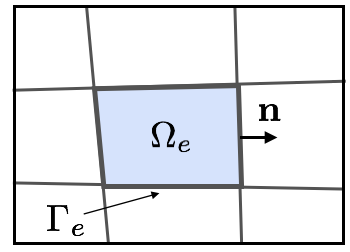
\includegraphics[width=1.5in]{DG_domain.png}
\label{fig:spatial_discretization/dg_domain}}
\subfigure[Element $\Omega_e$]{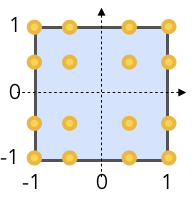
\includegraphics[width=1.5in]{DG_element.png}
\label{fig:spatial_discretization/dg_element}}
\end{center}
\caption{The (a) global domain and (b) element ($N=3$) for the DG method.}
\label{fig:spatial_discretization/dg_method}
\end{figure}

To construct discrete approximations of continuous differential operators (e.g., gradient, divergence, or curl) with the DG method, we first must represent the solution vector (call it $q$) using a polynomial representation.  That is, we represent the solution vector inside of each element $\Omega_e$ as follows
\be
q^{(e)}_N(\vec{x},t) = \sum_{i=1}^{M_N} \psi_i(\vec{x}) q^{(e)}_i(t)
\label{eq:spatial_discretization/dg_method}
\ee
where $\psi(\vec{x})$ are the known basis functions and $q^{(e)}_i(t)$ is the solution at each degree of freedom which will be time-dependent.
The superscript $(e)$ represents the specific element we are working with, $i=1,\ldots,M_N$ represents degrees of freedom inside each element $\Omega_e$.  Figure \ref{fig:spatial_discretization/dg_domain} shows a sample global domain whereby we then identify one specific element $\Omega_e$ to work with.  We then map the element from its physical space to the reference element presented in Fig.\ \ref{fig:spatial_discretization/dg_element}; in this particular example $M_N=(N+1)^2$ where $N=3$ which means we are using 3rd degree polynomials in each direction (yielding 4th degree accuracy).  In general, $N$ need not be constant in each direction and so we can also write $M_N=(N_{\xi}+1)(N_{\eta}+1)$ in two dimensions or $M_N=(N_{\xi}+1)(N_{\eta}+1)(N_{\zeta}+1)$ in three dimensions, where $\xi$ is along the horizontal direction, $\eta$ along the vertical, and $\zeta$ coming out of the page. 

The attraction of using basis functions $\psi$ to represent the solution $q$ is that computing the gradient of $q$ now only requires applying the gradient operator directly to Eq.\ \eqref{eq:spatial_discretization/dg_method} which yields
\be
\nabla q^{(e)}_N(\vec{x},t) = \sum_{i=1}^{M_N} \nabla \psi_i(\vec{x}) q^{(e)}_i(t)
\label{eq:spatial_discretization/dg_method/gradient}
\ee
where we are able to construct $\grad \psi$ \emph{a priori} since we have chose $\psi$ and these basis functions do not change in time (unless p-refinement is used which we will not consider here).

\subsubsection{DG Representation of Conservation Laws}
To describe the DG method, let us use it to represent the divergence operator for the conservation law
\be
\diff{q}{t} + \nabla \cdot \vec{f} = 0
\label{eq:spatial_discretization/DG_divergence/conservation_law}
\ee
where, in two dimensions, $f$ has components $\vec{f}=f_x \wh{\vec{i}} + f_y \wh{\vec{j}}$.
To construct a discrete approximation to Eq.\ \eqref{eq:spatial_discretization/DG_divergence/conservation_law} we first multiply by a test function $\psi_i$ and integrate within each element $\Omega_e$ as follows
\be
\inte \psi_i \diff{q^{(e)}_N}{t} d\Omega_e + \inte \psi_i \nabla \cdot \vec{f}^{(e)}_N d\Omega_e= 0.
\label{eq:spatial_discretization/DG_divergence/conservation_law/discrete}
\ee
Using the product rule, the second term can be written as follows
\be
\inte \psi_i \diff{q^{(e)}_N}{t} d\Omega_e + \inte \nabla \cdot \left( \psi_i \vec{f}^{(e)}_N \right) d\Omega_e - \inte \nabla \psi_i \cdot \vec{f}^{(e)}_N d\Omega_e= 0
\label{eq:spatial_discretization/DG_divergence/conservation_law/discrete2}
\ee
and invoking the divergence theorem for the second term yields
\be
\inte \psi_i \diff{q^{(e)}_N}{t} d\Omega_e + \intb \psi_i \nvector \cdot \vec{f}^{(e)}_N d\Gamma_e - \inte \nabla \psi_i \cdot \vec{f}^{(e)}_N d\Omega_e= 0
\label{eq:spatial_discretization/DG_divergence/conservation_law/discrete3}
\ee
where $\Gamma_e$ is the boundary of the element $\Omega_e$ and $\nvector$ is its outward pointing normal vector. We now need to fix the inconsistency of the second term above because it says that the solution along each element boundary $\Gamma_e$ is different from its neighbor since $\vec{f}^{(e)}_N$ is allowed to be discontinuous across element boundaries.  To fix this, we introduce a numerical flux such that what flows from element $\Omega_e$ to its neighbor $\Omega_k$ is the negative of what flows from $\Omega_k$ into $\Omega_e$.  We represent this fix as follows
\be
\inte \psi_i \diff{q^{(e)}_N}{t} d\Omega_e + \intb \psi_i \nvector \cdot \vec{f}^{(*,e)}_N d\Gamma_e - \inte \nabla \psi_i \cdot \vec{f}^{(e)}_N d\Omega_e= 0
\label{eq:spatial_discretization/DG_divergence/conservation_law/discrete4}
\ee
where $\vec{f}^{(*,e)}_N$ is the numerical flux that takes into account the solution at $\Omega_e$ and all its neighbors $\Omega_k$ represented by $\Gamma_e$.  In two dimensions we will have 4 face neighbors and in three dimensions we will have 6 face neighbors.  At this point one is free to choose their favorite numerical flux $\vec{f}^{(*,e)}_N$ just as one would do in the finite volume method (e.g., Rusanov, Roe, HLL, HLLC, etc.).  Note that it is the numerical flux term that couples all of the equations together; the rest of the terms are purely local within the element - this should be quite familiar for those of you coming from the finite volume community.

\subsubsection{Tensor Product Basis Functions}
In Eq.\ \eqref{eq:spatial_discretization/dg_method} we have said very little about the basis functions $\psi$ and have written the approximation in so-called monolithic form whereby all the degrees of freedom within an element are written as one long vector of length $M_N$.  This way of representing Eq.\ \eqref{eq:spatial_discretization/dg_method} allows for a quick explanation of the DG method but does not illustrate how the method is constructed when tensor product basis functions are used which is what we propose here.  In the case of tensor product basis functions, we rewrite $\psi$ (in 2D) as follows
\[
\psi_i(\xi,\eta) = h_j(\xi) \otimes h_k(\eta)
\]
where $h$ are one-dimensional basis functions, and $\otimes$ denotes the tensor (or Kronecker) product, and $j=1,\ldots N_{\xi}+1$, $k=1,\ldots,N_{\eta}+1$, and $i=j + (k-1) \left( N_{\xi}+1 \right)$. Using this strategy we can now rewrite Eq.\ \eqref{eq:spatial_discretization/dg_method} as follows
\be
q^{(e)}_N(\xi,\eta,t) = \sum_{i=1}^{N_{\xi}+1} \sum_{j=1}^{N_{\eta}+1} h_i(\xi) h_j(\eta) q^{(e)}_{ij}(t)
\label{eq:spatial_discretization/dg_method/tensor-product}
\ee
where we have written the approximation in terms of the reference element coordinates $(\xi,\eta$ instead of the physical coordinates $(x,y)$.  The advantage of doing this is that the reference element and its coordinates never change (assuming no p-refinement) which means that we can use one set of basis functions for all of the elements in the mesh.  

Taking the gradient of Eq.\ \eqref{eq:spatial_discretization/dg_method/tensor-product} yields
\be
\diff{}{\vec{x}} q^{(e)}_N(\xi,\eta,t) = \diff{}{\vec{x}} \sum_{i=1}^{N_{\xi}+1} \sum_{j=1}^{N_{\eta}+1} h_i(\xi) h_j(\eta) q^{(e)}_{ij}(t)
\label{eq:spatial_discretization/dg_method/tensor-product/gradient}
\ee
where $\vec{x}$ can represent either $x$ or $y$.  Let us look at each component separate and so invoking the chain rule yields
\[
\diff{}{x}=\diff{}{\xi} \diff{\xi}{x} + \diff{}{\eta} \diff{\eta}{x}
\]
and
\[
\diff{}{y}=\diff{}{\xi} \diff{\xi}{y} + \diff{}{\eta} \diff{\eta}{y}
\]
where the metric terms $\diff{\vec{\xi}}{\vec{x}}$ need to be computed for each element in the mesh.
Using these we can now rewrite Eq.\ \eqref{eq:spatial_discretization/dg_method/tensor-product/gradient} for the x-derivative as follows
\be
\diff{}{x} q^{(e)}_N(\xi,\eta,t) = \sum_{i=1}^{N_{\xi}+1} \sum_{j=1}^{N_{\eta}+1} \left( \diff{h_i(\xi)}{\xi}\diff{\xi}{x} h_j(\eta) + h_i(\xi) \diff{h_j(\eta)}{\eta}\diff{\eta}{x} \right) q^{(e)}_{ij}(t).
\label{eq:spatial_discretization/dg_method/tensor-product/x-deriv}
\ee
If we use the same polynomial order along $\xi$ and $\eta$ we can simplify Eq.\ \eqref{eq:spatial_discretization/dg_method/tensor-product/x-deriv} as follows
\be
\diff{}{x} q^{(e)}_N(\xi,\eta,t) = \sum_{i=1}^{N_{\xi}+1} \sum_{j=1}^{N_{\eta}+1} \left( dh_i \xi_x h_j + h_i dh_j \eta_x \right) q^{(e)}_{ij}(t).
\label{eq:spatial_discretization/dg_method/tensor-product/x-deriv2}
\ee
where $h$ is the basis function and $dh$ is its derivative, which are the same functions used along both directions $\xi$ and $\eta$; the index $(i,j)$ will account for which direction we are referring to.


\subsection{Time-Discretization Methods}

In order to circumvent the time-step restriction due to the fast moving acoustic waves, we will rely on implicit-explicit (IMEX) methods . For the LES model, if the aspect ratio of the horizontal to vertical grid spacing is near unity, it will be beneficial to use fully 3D-IMEX methods.  For the global atmospheric model, we propose to use 1D-IMEX methods whereby the time-integrator is fully explicit in the horizontal direction (HE) and implicit in the vertical direction (so-called HEVI schemes).

We propose to use a general family of additive Runge-Kutta methods (ARK) methods for both the 1D and 3D IMEX approaches (see, e.g., \citet{giraldo:2013} for 1D and 3D-IMEX methods based on ARKs). Note that adding fully-implicit Runge-Kutta (IRK) methods to the 3D-IMEX approach is quite trivial so this can be included as an option. Fully-implicit methods have no time-step restriction with respect to stability.

To get a sense of how the ARK approach works, let us partition the right-hand-side function $S(\vec{q})$ into its linear $L(\vec{q})$ and nonlinear $N(\vec{q})$ parts where the stiffness due to grid spacing or acoustic waves are contained in $L(\vec{q})$.  This then allow us to write the semi-discrete form (in space) as follows
\[
\diff{\qvector}{t} = L(\qvector) + N(\qvector) 
\]
which can now be discretized in time.  First we compute the stage values
\[
\vec{Q}^{(i+1)}=\qvector^n + \Delta t \sum_{k=0}^{i} \left( a_k N(\vec{Q}^{(k)}) \right) + \Delta t \sum_{k=0}^{i+1} \left( \wt{a}_k L(\vec{Q}^{(k)}) \right)
\]
with $i=0,\ldots,s$ where $s$ are the number of stages, $a$, and $\wt{a}$ are the coefficients of the double Butcher tableau defined in \citet{kennedy:2003,giraldo:2013}.  Additionally, 
$\vec{Q}^{(0)}=\qvector^n$ and the solution at time $n+1$ is obtained as follows
\[
\vec{q}^{n+1}=\qvector^n + \Delta t \sum_{k=0}^{s} \left( b_k S(\vec{Q}^{(k)}) \right)
\]
where the coefficients $b$ are also found in \citet{kennedy:2003,giraldo:2013}.
So far we have defined a diagonally-implicit Runge-Kutta (DIRK) method \citep{alexander:1977,butcher:1981a,ascher:1997,boscarino:2009}.  To make the DIRK more efficient, we impose the restriction that all the diagonal values $\wt{a}_{ii}$ to be constant. This allows one construction of the matrix problem which does not change across stage values.  This we now refer to as singly-diagonally-implicit Runge-Kutta (SDIRK).

\section{Topography}

\hl{Can we include a broad outline of how topography will be included already? I'd like to work from one high-resolution topography file, which may need to be coarse grained to the working resolution of the model.}

\section{Subgrid Scale Models}
\label{sec:sgs_models}

Subgrid-scale models for ``physics'' such as radiative transfer, microphysics, and convection parameterizations for coarse-resolution configurations are discussed in a separate document. Here we focus on SGS filters needed at any resolution, including LES resolutions \hl{(if we need them at all \dots).}


\section{Computing Aspects}
\label{sec:computing_aspects}

Let us decompose the computing aspects into the following groups
\begin{enumerate}
\item parallelization API
\item many-core API
\item graph-partitioning and grid generation

\end{enumerate}

\subsection{Parallelization API}
We propose to use the Message-Passing Interface (MPI) for communicating across processors and nodes (with multiple processors).  One of the NPS team members (Lucas Wilcox) has written Julia wrappers for MPI.

\subsection{Many-core API}
\label{sec:computing_aspects/manycore}
We propose to use a GPU library for accessing the GPUs. The NPS team has vast experience in this area. For example, the NPS team ported NUMA using OCCA2 with a CUDA back-end to run on the Titan supercomputer using 16,000 GPU cards achieving very good weak scaling \citep{abdi:2016b,abdi:2018}. The approach will be to write all of the compute-kernels in either GPUArrays (from Julia), OCCA2, or CUDA. From our perspective, the compute-kernel is the focus and most GPU-ready kernels look more or less the same (OCCA, CUDA, and OpenCL). 

\subsection{Graph-Partitioning and Grid Generation}
One of the NPS team members (Jeremy Kozdon) has written Julia wrappers to the p4est library developed by another NPS team member (Lucas Wilcox).  We propose to use p4est for both grid-generation and graph-partitioning or Metis with a specific grid generator for both the LES and global domains. The global domain will use a cubed-sphere grid while the LES domains will use a logically Cartesian cube grid.

\subsection{Code-base Repository}
The code is maintained in Github at \url{https://github.com/climate-machine/CLIMA}.

%-------Bibliography
\bibliographystyle{agufull08}
\bibliography{Giraldo_refs,CLIMA-refs}

\end{document}
